\section{Concept, Setup \& Implementation}

\subsection{Concept}
To build a functioning prototype, which implements the payment channel described in the previous chapter the following components are required:
\begin{enumerate}
    \item A supplier in form of a socket
    \item A customer in form of a plug
    \item A server to run a node that connects to the Ethereum blockchain
    \item A Smart Contract on the Ethereum blockchain
\end{enumerate}
All components will communicate with each other over a Wifi connection and TCP.
The following section will summarize all requirements each component of the prototype has to meet. An in depth explanation of the setup and technical implementation will follow in the next section.

\subsubsection{Socket}
An AC electrical socket is required. A microcontroller, which can be placed between the electrical circuit and the socket, needs two additional components: a WiFi module to communicate with the web and the plug and a relay to switch the current on and off.

\subsubsection{Plug}
An AC electrical plug is required, e.g. a short extension cord, that can be connected to any electronic device. A hall effect-based current meter can be attached to the hot wire to measure the current. This current meter needs to be attached to a microcontroller which also has a WiFi module to communicate with the socket and make http requests to the server.

\subsubsection{Server}
The server will run an Ethereum node. This node has to be reachable from the outside, so the microcontrollers can send http requests to it.

\subsubsection{Smart Contract}
The Smart Contract acts as a trustee, managing the money during the exchange. It has to be programmed in a way that guarantees that no party can steal from the other.

\newpage
\subsection{Setup}
This section will focus on the technical setup of the hardware components and the installation and setup of all required software.
\\
\subsubsection{Socket}
The Sonoff S20 smart socket was used for the technical implementation of the concept, as it meets all requirements listed in the section above. A microcontroller is automatically powered by the socket it’s plugged into. The S20 also has a WiFi module and a relay, which can be switched on and off by said microcontroller. Lastly the microcontroller can be reprogrammed via a serial port.
\\
\begin{figure}[h]
    \includegraphics[width=\textwidth]{img/S20_open.png}
    \caption{Sonoff S20}
    \label{fig:S20}
\end{figure}
\newpage
To program the microcontroller with a computer a FTDI USB to serial converter is required. The converter has to be plugged into the S20 as follows:
\\
\begin{center}
    \begin{tabular} { |c|c| }
        \hline
        FTDI Converter & Sonoff S20 \\
        \hline\hline
        GND & GND \\
        \hline
        TX & RX \\
        \hline
        RX & TX \\
        \hline
        3.3V & 3.3V \\
        \hline
    \end{tabular}
\end{center}
\leavevmode
\\
It's important to notice that the FTDI converter must operate at 3.3V entirely. Caution: some converters only switch the TX and RX pin to 3.3V while the VCC remains at 5V. This can fry the internals of the S20. To program the microcontroller, the button has to be pressed before plugging the pins into the serial port to put it in programming mode. After the pins have been inserted, the button can be released shortly after.
\\
\begin{figure}[h]
    \includegraphics[width=\textwidth]{img/serial_port.png}
    \caption{Serial ports of the Sonoff S20}
    \label{fig:S20_serial}
\end{figure}
\newpage
Both, the socket and the plug, will be programmed using the Arduino IDE. The following steps need to be followed to install the ESP8266 Board, which the S20 is based on:

\begin{itemize}
    \item Inside the Arduino IDE open "Preferences"
    \item Enter \url{http://arduino.esp8266.com/stable/package_esp8266com_index.json} under "Additional Boards Manager URLs"
    \item Open Tools $\rightarrow$ Board $\rightarrow$ Boards Manager
    \item Search and install "esp8266" by "ESP8266 Community"
\end{itemize}

After connecting the FTDI converter to the computer, it should appear under Tools $\rightarrow$ Port. To successfully flash code to the S20 the following settings have to be set:

\begin{itemize}
    \item Board: "Generic ESP8266 Module"
    \item CPU Frequency: "80 MHz"
    \item Flash Size: "1M (no SPIFFS)"
\end{itemize}
\leavevmode

\subsubsection{Plug}
The device to control the measurement of current in the plug and handle the communication with the socket is the Heltec WiFi Kit 8, which is based on an ESP8266 as well and has a 0.91 inch OLED display.
\\
\begin{figure}[h]
    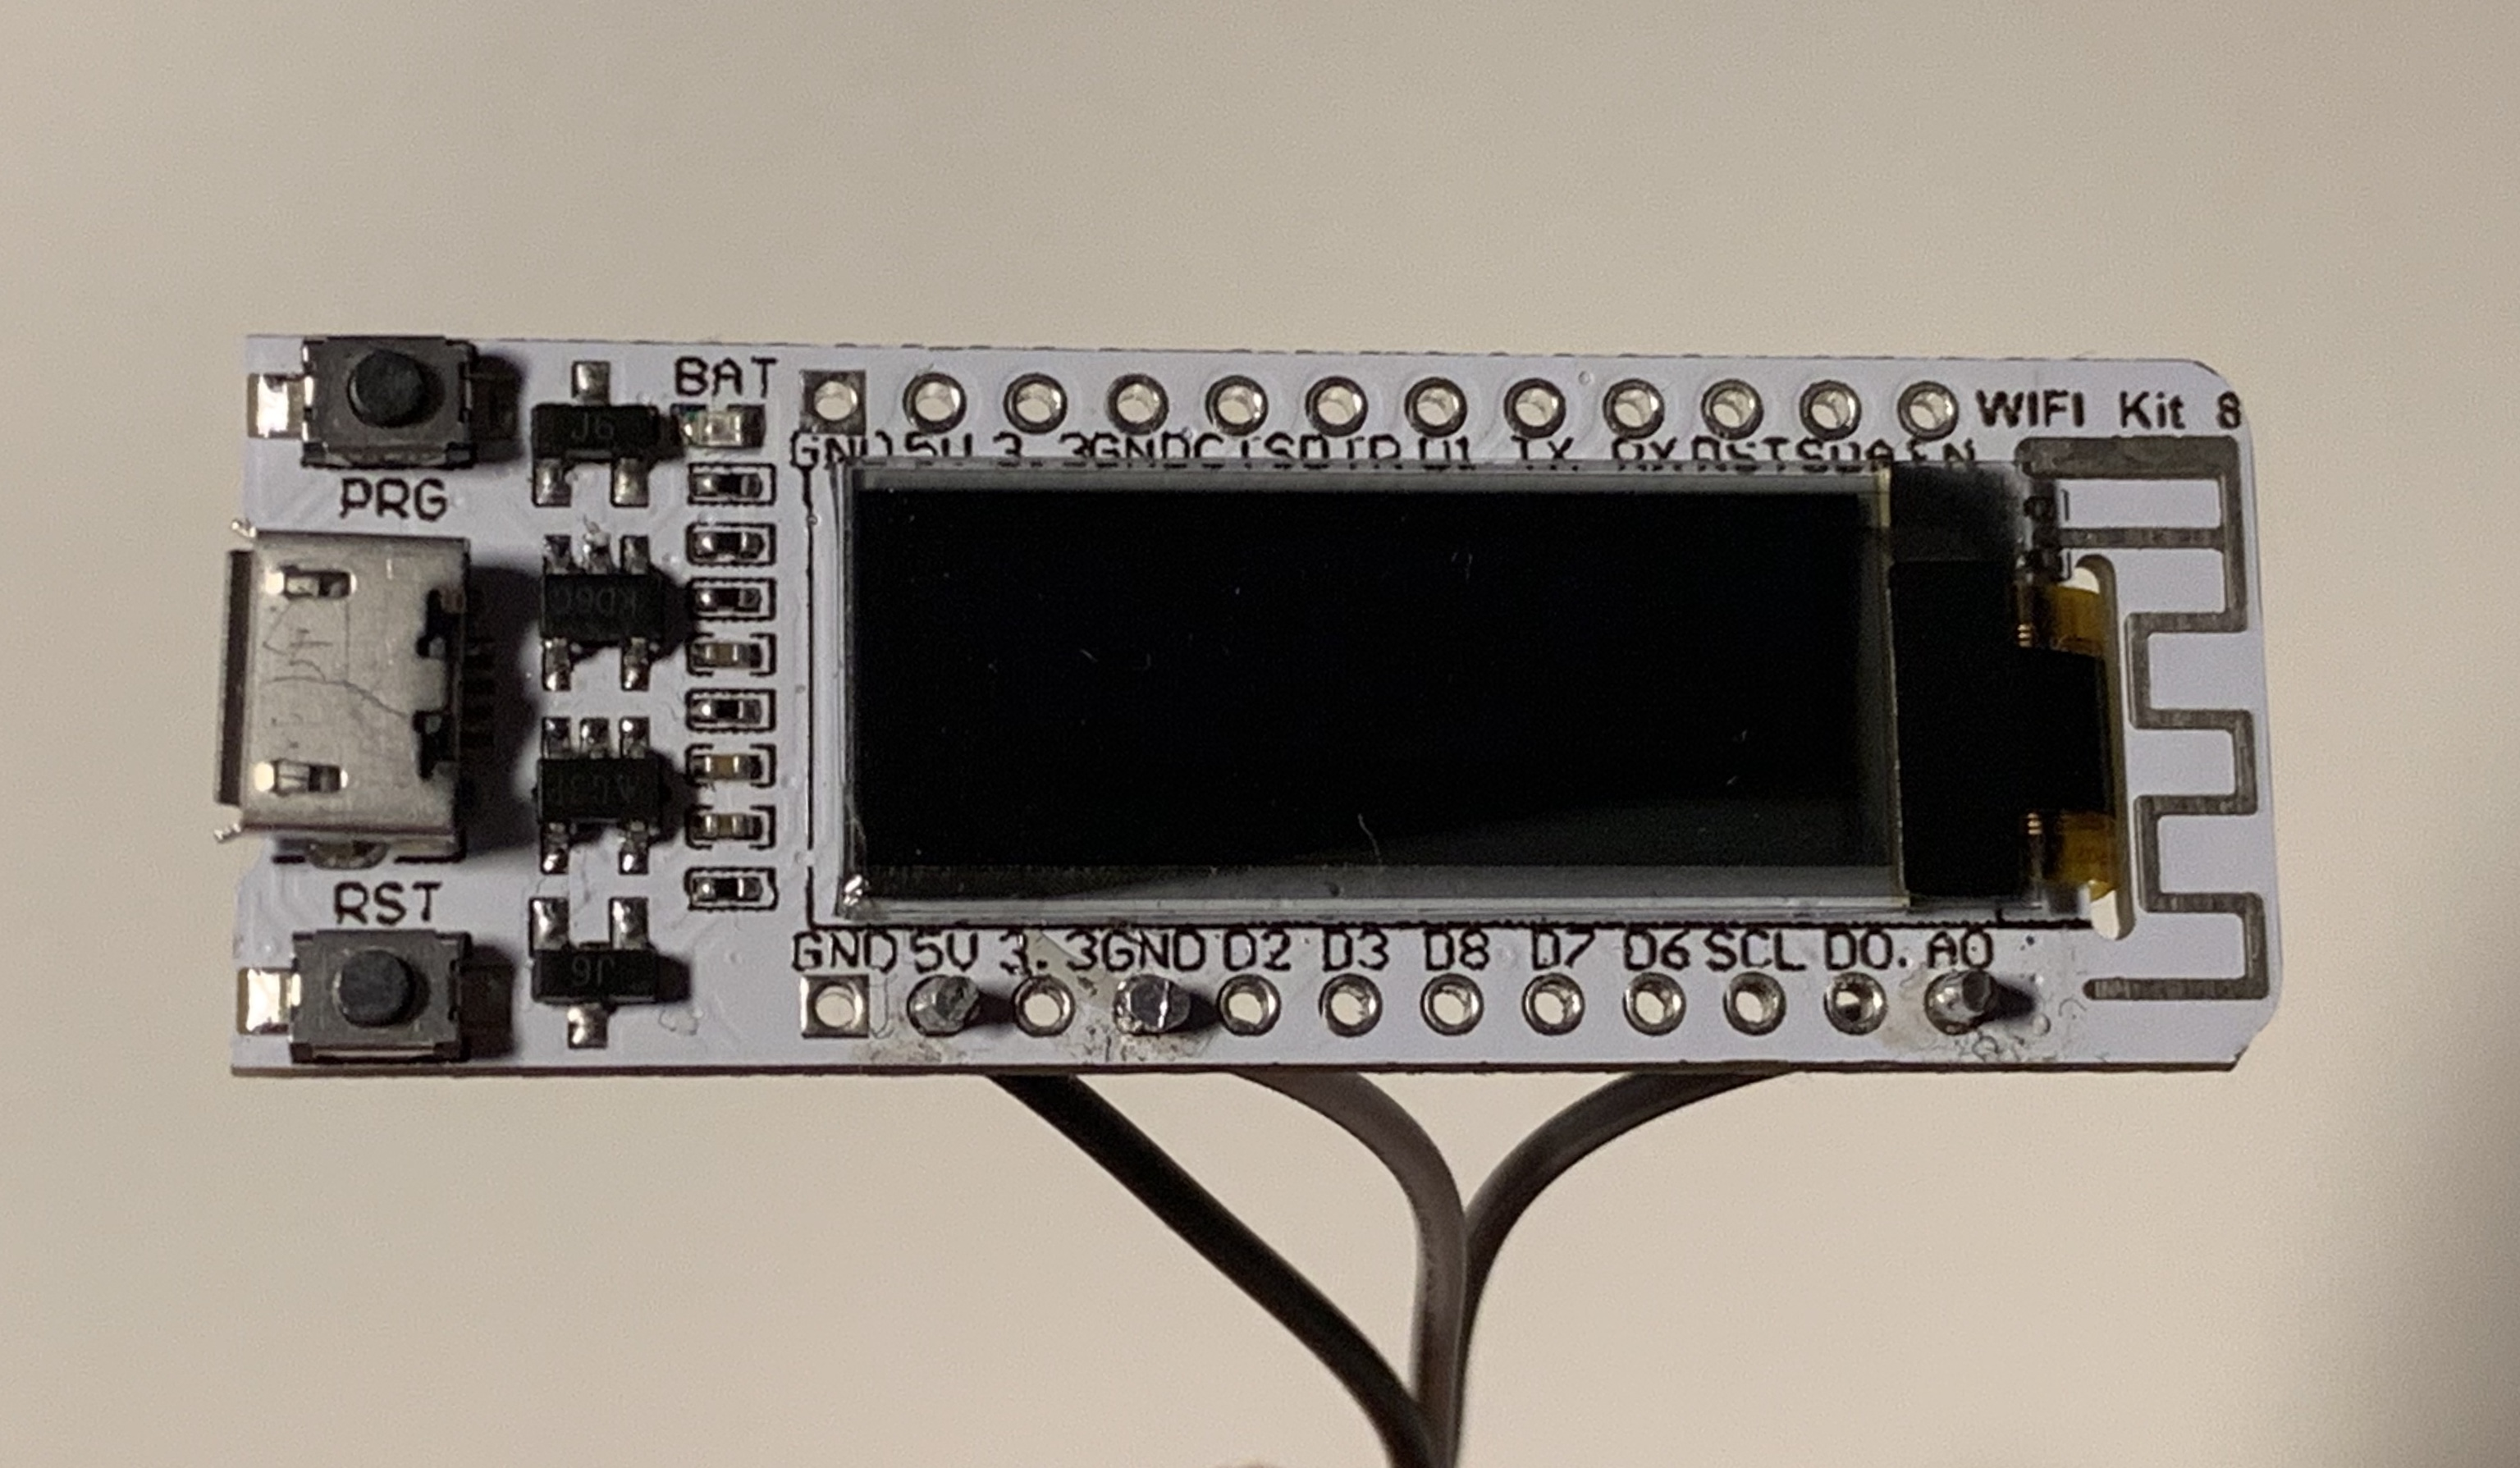
\includegraphics[width=\textwidth]{img/heltec.jpg}
    \caption{Heltec WiFi Kit 8}
    \label{fig:heltec}
\end{figure}

The ACS712 20A current meter is used to measure the current. It’s hall effect-based and provides galvanic isolation up to a minimum of 2.1 kV (RMS)\cite{acs712}. To connect the current meter, a part of the hot wire leading to the plug has to be cut and stripped. Both ends have to be inserted into the screw terminal of the ACS712. The current from the plug will now be redirected underneath the hall sensor.
\\
\begin{figure}[h]
    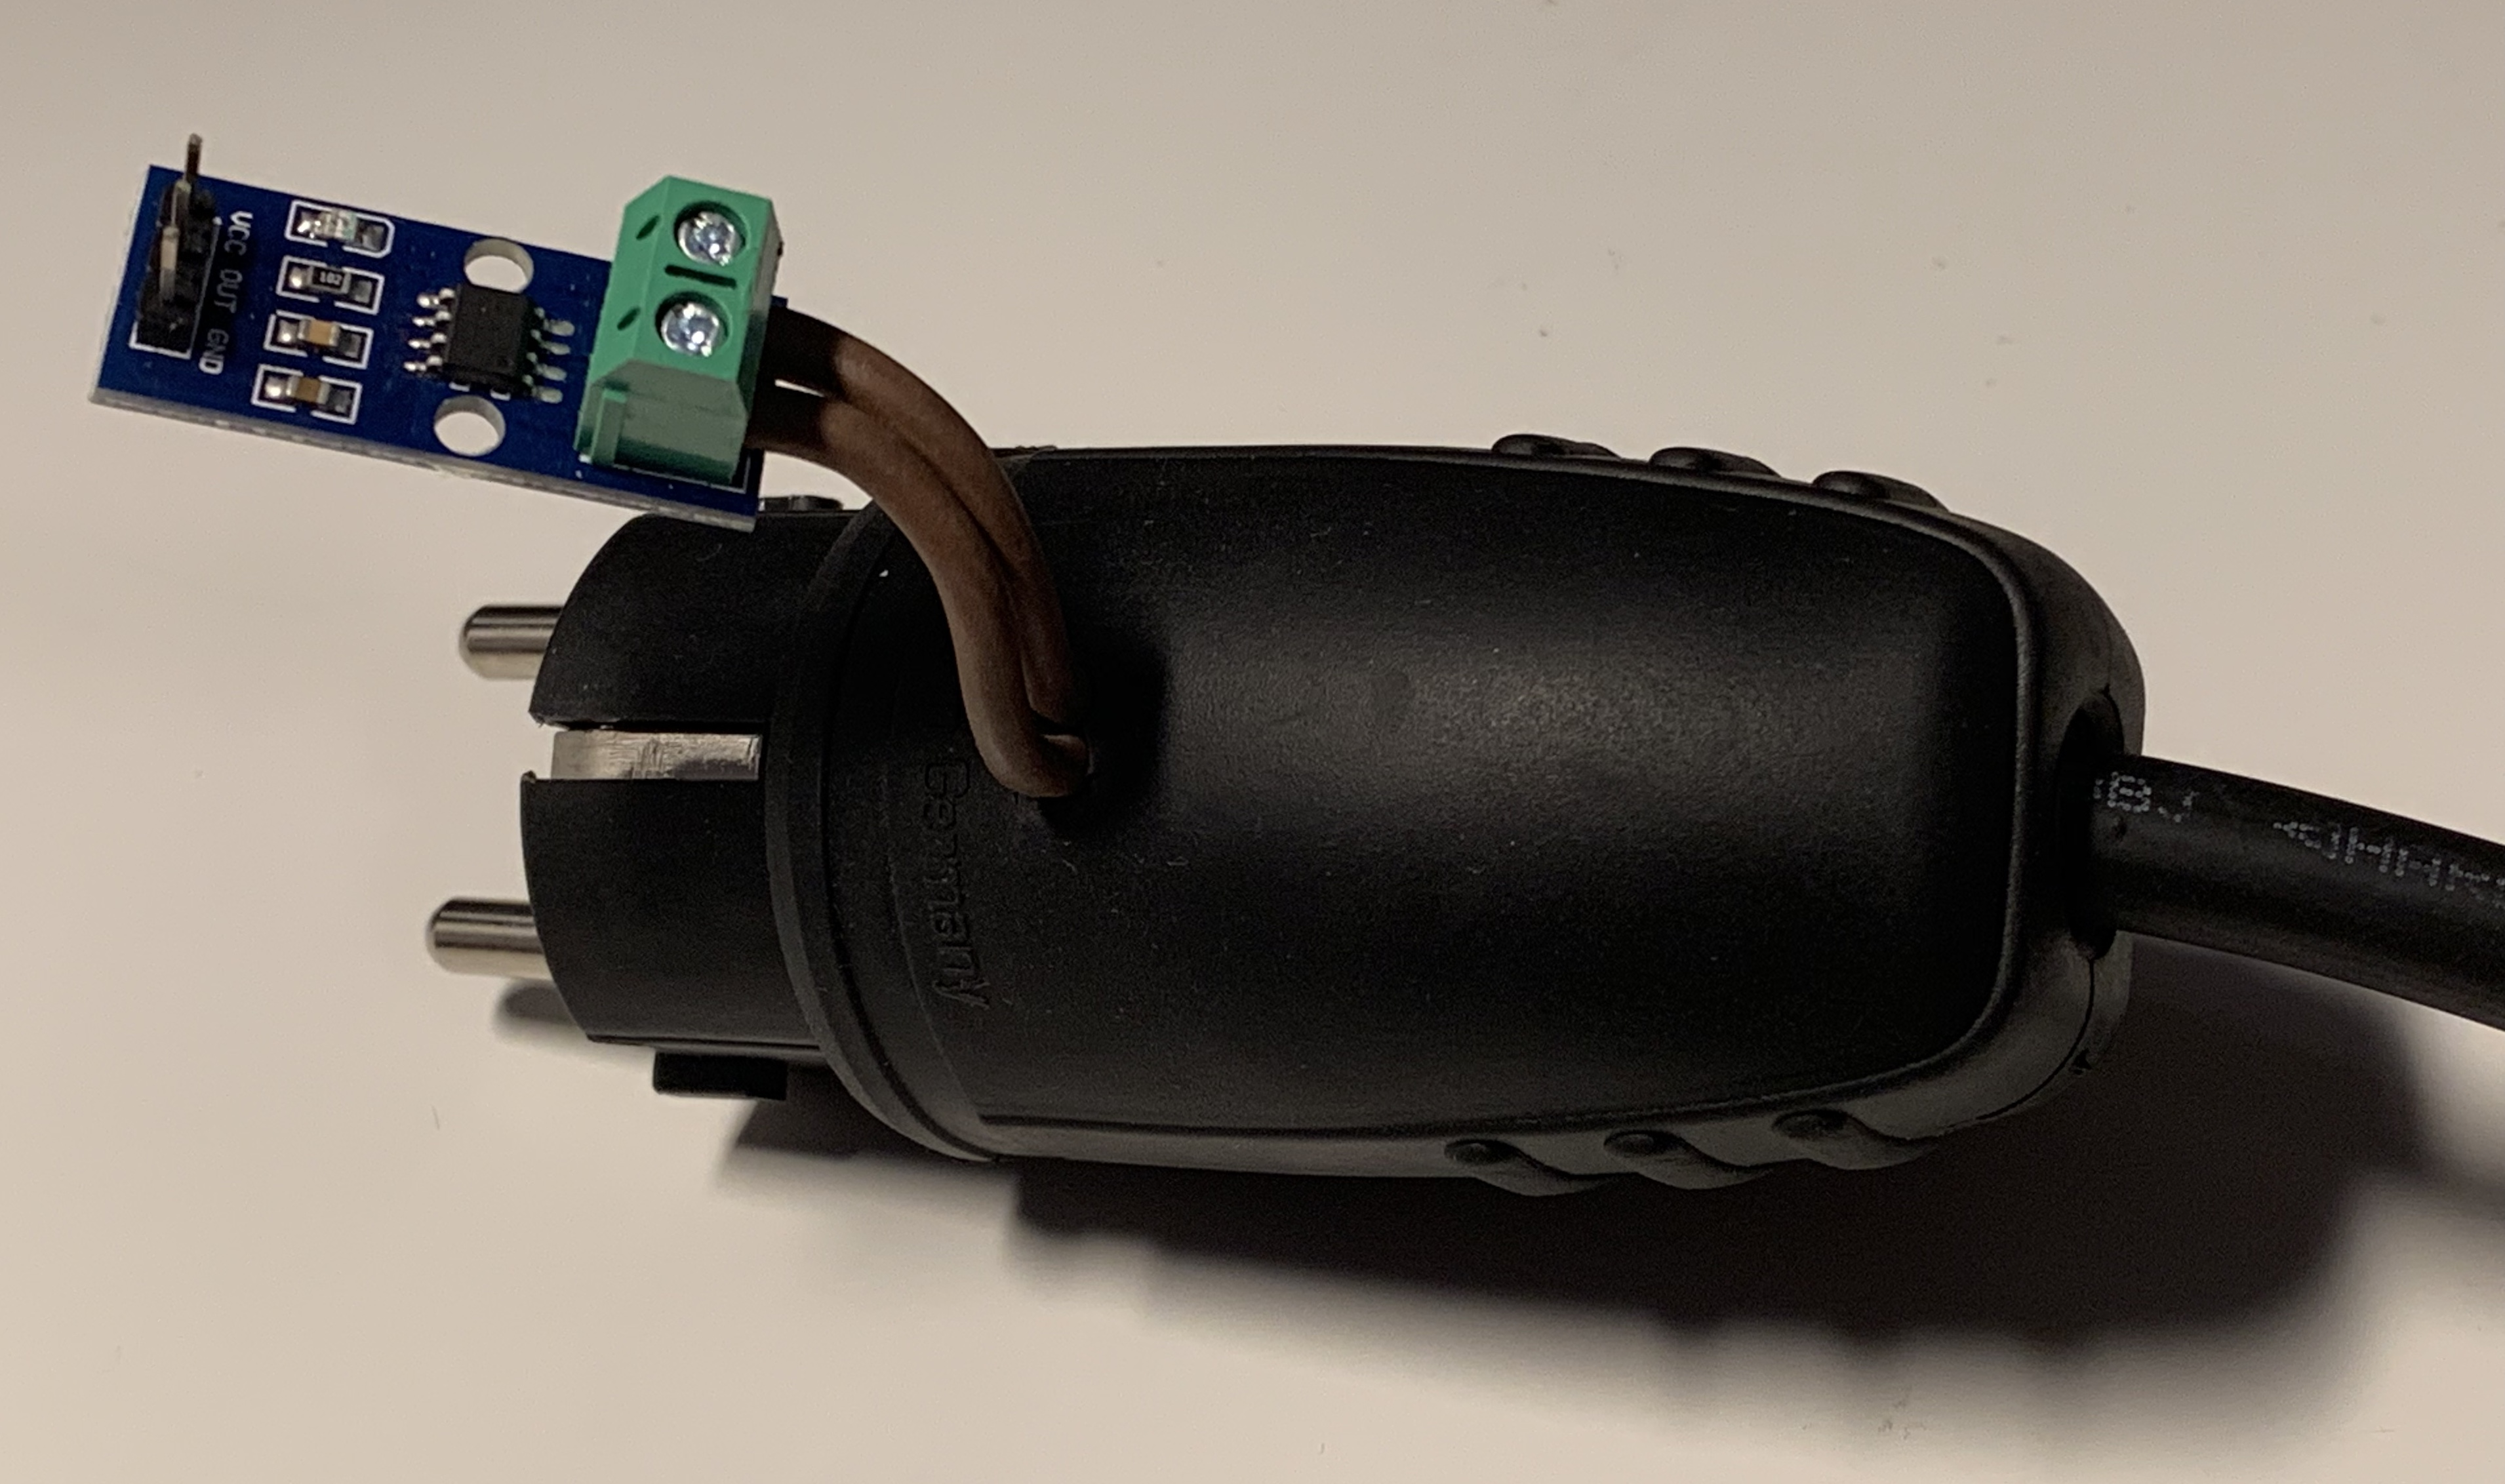
\includegraphics[width=\textwidth]{img/acs712.jpg}
    \caption{ACS712 current meter connected to plug}
    \label{fig:acs712}
\end{figure}

The pins of the current meter have to be soldered to the Heltec board as follows:
\\
\begin{center}
    \begin{tabular} { |c|c| }
        \hline
        ACS712 & Heltec WiFi Kit 8 \\
        \hline\hline
        VCC & 5V \\
        \hline
        OUT & A0 \\
        \hline
        GND & GND \\
        \hline
    \end{tabular}
\end{center}
\leavevmode
\\
To program the Heltec WiFi Kit 8, USB to UART drivers need to be installed first. The download link can be found under "References"\cite{vcp-drivers}. Next, if the ESP8266 was not installed inside the Arduino IDE yet, the instructions found in the section above can be used to install the board.
\\
After a successful driver installation, the board should be found under Tools $\rightarrow$ Port when the device is connected to the computer.
\newpage
The following settings are required to ensure a successful flash of the Heltec WiFi Kit:

\begin{itemize}
    \item Board: "NodeMCU 1.0 (ESP-12E Module)"
    \item CPU Frequency: "160 MHz"
    \item Flash Size: "4M (3M SPIFFS)"
\end{itemize}
\leavevmode

\subsubsection{Libraries}
The prototype relies on some external libraries that have to be installed additionally:
\\\\
\textbf{Display}\\
To use the display of the Heltec WiFi Kit a special library needs to be installed. Under Sketch $\rightarrow$ Include Library $\rightarrow$ Manage Library search for and install the "U8g2" library by "oliver".
\\\\
\textbf{WebSocket server}\\
The communication between the plug and the socket relies on WebSockets. Download the library as a zip file from the git repository\cite{websockets}.
\\
Install it via Sketch $\rightarrow$ Include Library $\rightarrow$ Add .ZIP Library.
\\\\
\textbf{ECDSA Library}\\
Ethereum relies on the Elliptic Curve Digital Signature Algorithm, although there are some differences to the standard implementation of that algorithm, which will be explained later. The zip library is provided with the source code of this prototype and extends the "micro-ecc" library by Kenneth MacKay\cite{micro-ecc}.
\\

\subsubsection{Server}
A server is mandatory to act as a gateway to the Ethereum blockchain. Geth is the official "Golang implementation of the Ethereum protocol"\cite{geth} and is used to run a full node. After the installation it will be used to send transactions and make smart contract calls.
\\\\
A \abbr{Virtual Private Server}{VPS} was used for this implementation running Ubuntu 18.04. The server has a six core CPU, 16 GB of RAM, 400GB SSD and 400 MBit/s unlimited traffic. The following instructions can be used to install the program under Ubuntu. For other environments the link to the instructions can be found under "References"\cite{geth-instructions}.
\newpage
To install geth add the repository first:
\begin{lstlisting}[language=bash]
  $ sudo add-apt-repository -y ppa:ethereum/ethereum
\end{lstlisting}

Next, install geth:
\begin{lstlisting}[language=bash]
  $ sudo apt-get update
  $ sudo apt-get install ethereum
\end{lstlisting}
\leavevmode
\\
To interact with the Ethereum Blockchain the entire chain history has to be downloaded first. This can take up to 40 GB of disk space and will take several hours of synchronizing. Geth will be started via this console command:
\begin{lstlisting}[language=bash, showstringspaces=false]
  $ geth console --rinkeby --rpc --rpcapi="db,eth,net,web3,
  personal,txpool" --rpcaddr X.X.X.X --rpcport 8545 --cache=1024
\end{lstlisting}

The launch options have the following purposes\cite{cli-options}:
\begin{itemize}
    \item rinkeby: synchronizes the Rinkeby testnet
    \item rpc: enables the HTTP-RPC server, allows to receive JSON RPC requests
    \item rpcapi: exposed APIs, listing of all APIs can be found under "References"\cite{json-rpc}\cite{management-apis}
    \item rpcaddr: IP address of RPC interface, replace "X.X.X.X" with the IP address of the server, defaults to "localhost". Exposing the RPC interface without any restrictions is not advisable, especially on the mainnet, as it’s a severe security concern.
    \item rpcport: listening port of the RPC server
    \item cache: memory allocated in MB, a minimum of 1024 MB is advisable for a faster synchronization
\end{itemize}
The console parameter starts a JavaScript console, allowing to interact with the blockchain using the web3 library. Geth currently comes with web3 version 0.20.1\cite{javascript-0.20} but might be upgraded to version 1.0\cite{javascript-1.0} soon. The links to the documentation of both versions can be found under "References".
\\
The version of the web3 library can be checked using:

\begin{lstlisting}[language=bash]
  > web3.version
\end{lstlisting}

The output of the synchronization could hamper the ability to properly read the output of the JavaScript console. The verbosity can be set via the following command:

\begin{lstlisting}[language=bash]
  > debug.verbosity(x)
\end{lstlisting}

Replace x with 0 for silent, 1 for error, 2 for warn, 3 for info, 4 for debug and 5 for detail. The verbosity defaults to info\cite{cli-options}.
\newpage

\begin{lstlisting}[language=bash]
  > eth.blockNumber
\end{lstlisting}

returns the block number of the latest synchronized block, which is the amount of all previous blocks. The first block, the also called the genesis block, starts with the block number 0. The current block number can be checked through so-called block explorers, e.g. {rinkeby.etherscan.io}.
\\
\begin{lstlisting}[language=bash]
  > eth.syncing
\end{lstlisting}
returns the current block number and the highest block number. As soon as the client is synchronized it returns "false"\cite{javascript-0.20}.


\subsubsection{Smart Contract}
\paragraph{Wallet}
The first thing needed to start programming smart contracts is an Ethereum wallet. MetaMask is a browser extension for Chrome, Firefox and Opera, that not only allows to manage multiple accounts on multiple test chains, it also injects the web3.js library into websites allowing to interact with the Ethereum blockchain and smart contracts on web pages.
Visit the MetaMask\cite{metamask} website and download the browser extension. A new account will be generated using a mnemonic phrase, defined in the BIP39 (Bitcoin improvement proposal)\cite{bip39}. It usually consists of 12 words which represent a private key, essentially creating an easy way to remember / write down private keys. An example for a mnemonic phrase is:
\begin{lstlisting}[language=bash]
  short heavy hidden anger nephew tragic
  fade dad renew finger among tiny
\end{lstlisting}
This phrase translates to the following seed:
\begin{lstlisting}[language=bash]
  b7b36d9ca1e105045344ecb7ca7b9449bfc0889139c9719876d03cf7b5814
  86137e905b9e94e50c03ca22871937ae3c754dea1427eede8198c6774d90f
  c1a1f4
\end{lstlisting}

Using the BIP44\cite{bip44} standard an unlimited amount of private keys can be derived from the seed. For example the first private key derived from this seed would be:
\begin{lstlisting}[language=bash]
  0xfb8502c03ea336344dc44b66b1a3c01e
    2917138e92bfa93c54725166394cd46b
\end{lstlisting}
with the corresponding address
\begin{lstlisting}[language=bash]
  0x4d43c1E254a9333fB0D8A50BD3f01b6787ee8895
\end{lstlisting}
The second derived private key is:
\begin{lstlisting}[language=bash]
  0x64b45c024041178aff2f9ed7b7026fff
    6890c871818c39c1c7bd826e6aa33773
\end{lstlisting}
\newpage
with the corresponding address
\begin{lstlisting}[language=bash]
  0xd38F7dc2d9B6F6D9d5CB6C8813e213D5DC541458
\end{lstlisting}
and so on. This means that the single mnemonic phrase will act as a backup phrase for all accounts that will be created inside the MetaMask wallet.
After MetaMask was set up create a second account and set the network to Rinkeby.
\paragraph{Getting Ether}
The next step would be to get Ethers on the Rinkeby network to interact with the Blockchain, via the website faucet.rinkeby.io. A public Facebook post or Twitter tweet containing the desired destination address has to be provided to receive the Ethers.

\paragraph{IDE}
The Smart Contract was developed using the Remix. It’s an online IDE including a compiler for the language Solidity, various debugging and testing tools and can be found under remix.ethereum.org.
\\
First a compiler has to be set inside the "Compile" tab. Because the programming language was designed especially for Ethereum, it is still under very heavy development with frequent updates coming out. The documentation for each specific version can be found under
\\
\url{https://solidity.readthedocs.io/en/v0.5.8/}
\\
while replacing "0.5.8" (the latest stable version at the time of writing) with the desired compiler version.
\\\\
Inside the "Run" tab the connection to the blockchain can be chosen under "Environment". The most important options are:
\begin{itemize}
    \item JavaScript VM: A personal Ethereum blockchain implemented in JavaScript that runs locally. It comes with 5 accounts which are preloaded with 100 Ether. It’s suited for early development stages, unit testing, and all in all quick tests, as there are no transaction times.
    \item Injected Web3: As mentioned before, MetaMask injects Web3 into websites. When choosing this option, the currently active account and the chosen network in MetaMask are used for development.
\end{itemize}
Underneath the Smart Contract can be chosen and deployed to the blockchain. Next to the deploy button, constructor arguments can be passed. Optionally an existing Smart Contract can be loaded from an address.
\\\\
After a Contract has been deployed or loaded, all functions and public variables will be listed under the "Deployed Contracts" section. This will be the main way to interact with the Smart Contract.